\subsection{Neural Networks}
Neural networks are built upon a simplified understanding of how the neurons in the brain function, wherein electrical impulses are passed in a chain reaction throughout the brain.
Feed-forward neural networks typically model this by passing an input through a composition of linear transformations and non-linear activation functions.
In a so-called \textit{feed-forward pass}, the input values $\boldsymbol{x} \in \mathbb{R}^{N_0}$ are sent to each neuron in the next layer, multiplied by a predetermined weight along the way with a value added called the bias $\boldsymbol{b} \in \mathbb{R}^{N_1}$.
We represent this through the function $\mathcal{A} : \mathbb{R}^{N_{i-1}} \to \mathbb{R}^{N_{i}}$ defined by
\begin{equation}\label{eq:A_func}
    \mathcal{A}_i(\boldsymbol{x}) = W_i \boldsymbol{x} + \boldsymbol{b}_i,
\end{equation}
where $W \in \mathbb{R}^{N_i \times N_{i-1}}$ is the weight matrix, where the $N_i$ is the number of neurons in layer $i$.
The resulting values are denoted $\boldsymbol{z}^i$.

The result of this is then passed through an activation function $\sigma_i : \mathbb{R} \to \mathbb{R}$, which we apply element-wise by $\boldsymbol{a}^i_j = \sigma_i (\boldsymbol{z}^i_j)$.
To simplify notation, we simply notate this as $\boldsymbol{a}^i = \sigma_i(\boldsymbol{z}^i)$.
This continues throughout each layer, culminating in the output layer, which in our case will simply have a the identity function as its activation function.
This process is illustrated in \autoref{fig:SimpleFFNN}.

\begin{figure}[h]
\centering
\def\layersep{2.5cm}
\def\nodeinlayersep{1.2cm}
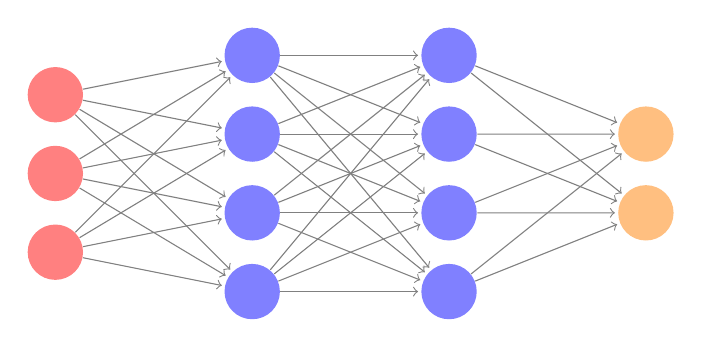
\begin{tikzpicture}[shorten >=1pt,->,draw=black!50, node distance=\layersep]
    \tikzstyle{every pin edge}=[<-,shorten <=1pt]
    \tikzstyle{neuron}=[circle, fill=black!25,minimum size=20pt,inner sep=0pt]
    \tikzstyle{input neuron}=[neuron, fill=red!50];
    \tikzstyle{output neuron}=[neuron, fill=orange!50];
    \tikzstyle{hidden neuron}=[neuron, fill=blue!50, minimum size=20pt];
    \tikzstyle{hidden neuron2}=[neuron, fill=blue!50, minimum size=20pt];

    \foreach \name / \y in {0,...,2}
        \node[input neuron] (I-\name) at (0,-\y) {};

    \foreach \name / \y in {0,...,3}
        \path[yshift=0.5cm]
            node[hidden neuron] (H1-\name) at (\layersep,-\y cm) {};

    \foreach \name / \y in {0,...,3}
        \path[yshift=0.5cm]
            node[hidden neuron2] (H2-\name) at (2*\layersep,-\y cm) {};    

    \foreach \name / \y in {0,...,1}
        % \node[output neuron,pin={[pun edge={->}]right:Output \#\y}, right of=H2-2] (O-\name) at (3*\layersep, -\y cm) {};
        \path[yshift=-0.5cm]
            node[output neuron] (O-\name) at (3*\layersep, -\y cm) {};


    \foreach \source in {0,...,2}
        \foreach \dest in {0,...,3}
            \path (I-\source) edge (H1-\dest);

    \foreach \source in {0,...,3}
        \foreach \dest in {0,...,3}
            \path (H1-\source) edge (H2-\dest);

    \foreach \source in {0,...,3}
        \foreach \dest in {0,...,1}
            \path (H2-\source) edge (O-\dest);
\end{tikzpicture}
\caption{Illustration of a fully connected feed-forward neural network with an input layer (teal), two hidden layers (purple) and an output layer (beige).}
\label{fig:SimpleFFNN}
\end{figure}

Let $\boldsymbol{\theta} = \{ W_i, \boldsymbol{b}_i \}_{i = 1}^L$ represent the trainable parameters of the network in the parameter space $\mathcal{V}$, and $\mathcal{N}_{\boldsymbol{\theta}} : \mathbb{R}^{N_0} \to \mathbb{R}^{N_L}$ denote the realization of a neural network with $L$ layers, defined through the composition
\begin{equation}\label{eq:NNreal}
\begin{split}
    \mathcal{N}_{\boldsymbol{\theta}} &= \sigma_L \circ \mathcal{A}_L \circ \sigma_{L-1} \circ \ldots \circ \sigma_{1} \circ \mathcal{A}_1 \\
    &= \compfunc_{i = 1}^L \sigma_i \circ \mathcal{A}_i.
\end{split}
\end{equation}
We call the parameters trainable, as we typically initialize them to random values, \textit{training} them through optimization with the help of the backpropagation algorithm.
We do this by measuring how well our model is able to predict a set of values with a cost function $\mathcal{C}$, which often gives the problem the form of finding
\begin{equation}\label{eq:argmintheta}
    \hat{\boldsymbol{\theta}} = \argmin_{\boldsymbol{\theta} \in \mathcal{V}} \mathcal{C} \left( \mathcal{N}_{\boldsymbol{\theta}}, \boldsymbol{x}, \boldsymbol{\hat{y}} \right),
\end{equation}
where $\boldsymbol{\hat{y}} \in \mathbb{R}^{N_L}$ are a set of target values.

A typical choice of $\mathcal{C}$ in a regression problem is the Mean Squared Error (MSE), defined by
\begin{equation}
    \mathcal{C}(\mathcal{N}_\theta, \boldsymbol{x}, \boldsymbol{y}) = \frac{1}{n} \lVert \mathcal{N}_\theta(\boldsymbol{x}) - \boldsymbol{y} \rVert_2^2.
\end{equation}
One of the main benefits of this measure is its ease of differentiation, lightening the computational load of training the network.

Through the Universal Approximation theorem, first proven by \textcite{Cybenko1989ApproximationBS} and since extended, neural networks have a proven capacity to approximate any given function.
It does not state however how one is to find the architecture and parameters which solve a given problem.
The theorem does however guarantee the validity of at least attempting to utilize neural networks in a number of fields.

\subsection{Partial Differential Equations}
A Partial Differential Equation (PDE) is defined to be an equation containing a function with at least two different variables, as well as some degree of partial derivatives to these variables.
PDEs are ubiquitous in describing the properties, behavior, and evolution of physical systems.

An important concept when discussing PDEs is differential operators.
A differential operator is defined as a function performing some sort of differentiation on the function it is applied to.
It is indeed a function from a function space $\mathcal{F}_1$ to another function space $\mathcal{F}_2$.
In the case of a function of $n$ variables $u(x_1, x_2, \ldots , x_n)$ the usual differential operator is defined as 
\begin{equation*}
    D^\alpha u = \frac{\partial u^{|\alpha|}}{\partial x_1^{\alpha_1} \partial x_2^{\alpha_2} \cdots \partial x_n^{\alpha_n}},
\end{equation*}
where $|\alpha| = \alpha_1 + \alpha_2 + \ldots + \alpha_n$.
When considering a function $u(x,y)$, we will denote $\frac{\partial u}{\partial x}$ as $u_x$, $\frac{\partial^2 u}{\partial x^2}$ as $u_{xx}$, and so on.
We will when discussing general PDEs denote the differential operator characterizing the PDE by $\mathcal{L}$.

An example of a PDE is Poisson's equation, which is characterized by
\begin{equation*}
    u_{xx} + u_{yy} = f \text{ on }\Omega,
\end{equation*}
where the residual $f$ is independent of $u$, on the domain $\Omega \in \mathbb{R}^d$, where $d$ is the number of dimensions.
In the 2D case, we have $\mathcal{L}u = u_{xx} + u_{yy}$, so that the equation can be denoted succinctly as $\mathcal{L}u = f$.

We will also come across the differential operator $\nabla$.
For a problem in three physical dimensions, $\nabla$ is defined as $\nabla = \frac{\partial}{\partial x}\boldsymbol{x} + \frac{\partial}{\partial y}\boldsymbol{y} + \frac{\partial}{\partial z}\boldsymbol{z}$, where $\boldsymbol{x},\boldsymbol{y},\boldsymbol{z}$ are the three-dimensional Euclidean unit vectors.

When considering time-dependent PDEs for physical problems, we frequently require initial and boundary conditions.
Initial conditions are conditions for values at $t=0$, and boundary conditions are conditions on the physical boundaries of the problem.
Thus, both conditions are defined on the boundary $\partial\Omega$ of our spatial-temporal domain, and we treat them similarly.
In this paper we encounter Dirichlet-type boundary conditions, where the value of the function on the boundary is given.
We return to the Poisson equation as an example;
we have for the function $u(x,y)$, $(x,y) \in [0,1]\times [0,1]$, the boundary conditions $u(0,y)=u(1,y)=u(x,0)=u(x,1) = 0$.
Neumann boundary conditions are also ubiquitous. This is when the boundary conditions determine the first order derivative in the direction normal to the boundary. 

To capture these boundary conditions, we introduce a boundary value operator $\mathcal B$ such that we can write $\mathcal B u = g$ on $\partial \Omega$ for all our boundary conditions, for some function $g$ on the boundary $\partial\Omega$.
Given the PDE operator $\mathcal L$ and the boundary value operator $\mathcal B$, we present the general form of a PDE as
\begin{equation}
\begin{cases}
    \mathcal{L}u = f &\text{in } \Omega,\\
    \mathcal{B}u = g &\text{in } \partial\Omega.
\end{cases}
\label{eq:PDE}
\end{equation}

\subsection{Physics-Informed Neural Networks}
Physics-Informed Neural Networks (PINNs) incorporate the inherent physical constraints of a problem directly into the network.
One such way is to bake in the PDE conditions of a problem directly into the loss function of the network \cite{RAISSI2019686}.
In doing so, we coerce the network into predicting results which adhere to the inherent physical laws.
In this way, we reduce the need for labeled data, and are able to be more confident in the predictions of our network.
Our neural network $\mathcal{N}_{\boldsymbol{\theta}}$ can then be regarded as an approximation of the hidden function $u$, denoting it as $u^*$.

We then measure the loss through
\begin{equation}\label{eq:PINNMSE}
    \MSE = \MSE_d + \MSE_0 + \MSE_u + \MSE_f,
\end{equation}
where
\begin{equation*}
\begin{split}
    \underbrace{\MSE_d}_{\text{data}} &= \frac{w_d}{N_d} \sum_{i = 0}^{N_d} \left( u^*(x_d^i) - u_d^i \right)^2,  \\
    \underbrace{\MSE_0}_{\text{Initial}} &= \frac{w_0}{N_0} \sum_{i = 0}^{N_0} \left( u^*(x_0^i) - u_0^i \right)^2,  \\
    \underbrace{\MSE_u}_{\text{Boundary}} &= \frac{w_u}{N_u} \sum_{i = 0}^{N_u} \left( u^*(x_u^i) - g(x_u^i) \right)^2, \\
    \underbrace{\MSE_f}_{\text{Residual}} &= \frac{w_f}{N_f} \sum_{i = 0}^{N_f} \left( \mathcal{L}u^*(x_f^i) - f(x_f^i) \right)^2.
\end{split}
\end{equation*}
In this case, $(x_d^i,u_d^i)_{i=1}^{N_d}$ is a sample of data, $u_0^i$ is our initial condition, and $N_d,N_0,N_u,N_f$ is the number of data-, initial-, boundary-, and residual points on which the loss is calculated respectively. $w_d,w_0,w_u,w_f$ are the respective weights given to each loss. 
With this baseline, one can extend the loss function through appending more terms, if there are other conditions, such as periodicity, one would like to enforce.
Note that in $\MSE_f$, we are taking the derivative of the network itself with respect to its output.
This is done through the use of automatic differentiation, in much the same way the parameters are optimized, described further in \autoref{sec:autodiff}.

The $\MSE_d$ can also be dropped, leading to unsupervised training. However, unsupervised PINNs have been documented to be slower than traditional numerical methods for solving PDEs \cite{en16124558}.
Nevertheless, with a framework already set up, the process of setting up a PINN is quite simple, in contrast to developing a numerical algorithm.

The PINN framework therefore presents a simple methodology to incorporating knowledge about the systems we wish to solve into our neural network training. 
Moreover, PINNs also retain the data-based learning from machine learning models, allowing the user to train using existing data. 
This approach has made PINNs particularly suited for inverse problems. Inverse problems involve determining some parameters of our system using data, and are notoriously difficult for traditional methods \cite{Jagtap_2022,garay2023physicsinformed}.

\subsection{Extended Physics-Informed Neural Networks}
Extended Physics-Informed Neural Networks (XPINNs) is a generalized space-time domain decomposition algorithm for PINNs initially proposed in \textcite{Jagtap2020ExtendedPN}.
The key idea is to decompose the domain $\Omega$ into several subdomains $(\Omega_s)_s^N$ such that $\bigcup_{s=1}^{N_\mathrm{sd}}\Omega_s=\Omega$, as illustrated in \autoref{fig:subdomain_comp}.
The domain interfaces are given by $\Omega_i\cap \Omega_j = \partial\Omega_{ij},\, i\neq j$.
Each subdomain is then equipped with its own sub-PINN $u^*_s$, and the training and test points associated with its subdomain.

\begin{figure}[h]
\centering
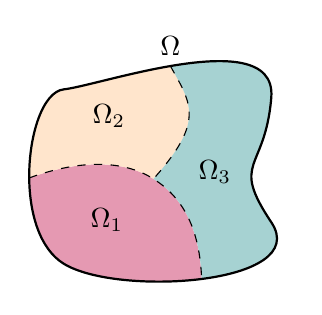
\begin{tikzpicture}[x=0.75pt,y=0.75pt,yscale=-1,xscale=1]

\coordinate (Top) at (283.69,109.1);
\coordinate (Left) at (215.67,163);
\coordinate (Bottom) at (298.76,211.69);
\coordinate (Middle) at (275.54,163.47);

\fill[purple!40] (Left) .. controls (240.17,154.14) and (260.97,154.24) .. (Middle) .. controls (290.11,172.69) and (297.8,187.76) .. (Bottom) .. controls (274.65,214.78) and (245.16,212.25) .. (232.3,204.34) .. controls (220.65,197.17) and (215.83,179.98) .. (Left) -- cycle;

\fill[orange!20] (Left) .. controls (215.47,142.06) and (222.36,121.44) .. (232.3,120.34) .. controls (240.46,119.43) and (262.42,112.76) .. (Top) .. controls (293.69,127.1) and (300.54,135.47) .. (Middle) .. controls (260.97,154.24) and (240.17,154.14) .. (Left) -- cycle;

\fill[teal!35] (Top) .. controls (309.31,104.7) and (333.94,104.67) .. (332.3,124.34) .. controls (329.3,160.34) and (312.3,154.34) .. (332.3,184.34) .. controls (342.4,199.5) and (323.39,208.53) .. (Bottom) .. controls (297.8,187.76) and (290.11,172.69) .. (Middle) .. controls (300.54,135.47) and (293.69,127.1) .. (Top) -- cycle;

\draw [thick]  (232.3,120.34) .. controls (240.46,119.43) and (262.42,112.76) .. (283.69,109.1) .. controls (309.31,104.7) and (333.94,104.67) .. (332.3,124.34) .. controls (329.3,160.34) and (312.3,154.34) .. (332.3,184.34) .. controls (342.4,199.5) and (323.39,208.53) .. (298.76,211.69) .. controls (274.65,214.78) and (245.16,212.25) .. (232.3,204.34) .. controls (220.65,197.17) and (215.83,179.98) .. (215.67,163) .. controls (215.47,142.06) and (222.36,121.44) .. (232.3,120.34) -- cycle ;
%Curve Lines [id:da968003923864855] 
\draw  [dashed]  (215.67,163) .. controls (240.17,154.14) and (260.97,154.24) .. (275.54,163.47) .. controls (290.11,172.69) and (297.8,187.76) .. (298.76,211.69) ;
%Curve Lines [id:da35316263230503897] 
\draw  [dashed]  (283.69,109.1) .. controls (293.69,127.1) and (300.54,135.47) .. (275.54,163.47) ;

% \node (A) at (Left) {};
% \node [rotate=-25, xshift=-0.5cm] (B) [left of=A] {Interface};
% \draw [thick,->] (B) edge (A);
\node [yshift=0.25cm] (C) at (Top) {$\Omega$};

% Text Node
\draw (244,176.4) node [anchor=north west][inner sep=0.75pt]    {$\Omega _{1}$};
% Text Node
\draw (296,153.4) node [anchor=north west][inner sep=0.75pt]    {$\Omega _{3}$};
% Text Node
\draw (245,126.4) node [anchor=north west][inner sep=0.75pt]    {$\Omega _{2}$};

\end{tikzpicture}
\caption{Domain decomposition of $\Omega$ into three subdomains $\Omega_i$, with dashed lines representing the interfaces $\partial \Omega_{ij}$. Each subdomain is equipped with its own unique PINN. }
\label{fig:subdomain_comp}
\end{figure}

Given such a domain decomposition, we now consider the following XPINN solution to our PDE problems:
\begin{equation}\label{eq:XPINN}
    u^* (x)=\sum_{s=1}^{N_\mathrm{sd}} u_{s}^*(x) \mathds{1}_{\Omega_s}(x),
\end{equation}
where $\mathds{1}_{\Omega_s}(x)$ is the indicator function given by:
\begin{equation}
    \mathds{1}_{\Omega_s}(x)=
    \begin{cases}
        0 &\text{If } x \notin \Omega_s \\
        1 &\text{If } x \in \Omega_s \backslash \text{common interface in } \Omega_s \\
        \frac{1}{S} &\text{If } x \in \text{common interface in } \Omega_s,
    \end{cases}
\end{equation}
where $S$ is the number of subdomains intersecting in the common interface.

A classical problem when applying domain decomposition is ensuring sufficient communication between the different subdomains such that their solutions reflect a global solution.
Ideally, the domain decomposition solution should be ``blind" to the decomposition.
For classical solvers, we frequently introduce \textit{ghost layers} to facilitate the communication between neighboring subdomains. 

However, as PINNs are mesh-independent we do not require ghost layers to communicate between PINNs.
XPINNs instead proposes to amend an additional \textit{interface loss} term $\MSE_I$ to the loss function \eqref{eq:PINNMSE} of each PINN to ensure that the PINNs agree on the subdomain interfaces.
For instance, we might wish to enforce continuity in our solution across an interface.
For a single PINN, we amend the loss function with
\begin{equation}\label{eq:MSE_I}
    \underbrace{\MSE_I}_{\text{Interface}} = \frac{1}{N_I} \sum_{i = 0}^{N_d} \left( u^*(x_I^i) - \{u_I^i\} \right)^2,  \\
\end{equation}
where $\{u_I^i\}$ is the average predicted value at the interface from each PINN, and $N_I$ is the number of points on the interface. 

Like traditional domain decomposition algorithms, XPINNs introduce an intuitive parallelization by separating the domain into several subdomains with their own respective neural network where the subdomain solutions can be computed on independent processors.
Thus, XPINNs might improve the computational efficiency through improved utilization of the processor architecture in a computer.

Moreover, \textcite{Jagtap2020ExtendedPN} argue that XPINNs also introduce architectural flexibility into our problem.
For instance, we might employ a deep network in a subdomain with complex solution, whereas we can apply a shallow network for a subdomain with relatively simple and smooth solutions. 

However, the domain decomposition introduces a tradeoff for generalization.
On the one hand, we can leverage the architectural flexibility of XPINNs to decompose a complex PDE solution into several simple parts, decreasing the problem complexity and boosting generalization.
On the other hand, decomposing leads to each subdomain having access to less training data, which might cause overfitting and worse performance overall.
However, in an unsupervised setting, the computational load can be balanced through introducing more points in a previously lighter subdomain.
For a more rigorous analysis of when XPINNs improve generalization, we refer the reader to \cite{XPINN_generalize}.

Furthermore, the interface conditions also introduce complications to the loss function, changing the loss landscape.
Thus, it is easy to imagine instances where for instance the loss landscapes of interface loss and boundary loss are different, resulting in an optimization dilemma of which condition to prioritize.
Moreover, changing the loss function through interface conditions might also correspond to altering the PDE problem equation.
To the extent of the authors' knowledge, there is not a clear theoretical understanding of how the interface conditions alter the solution to our PDE problem. 

\subsection{Automatic Differentiation}\label{sec:autodiff}
The backpropagation algorithm \cite{Backpropogation1986} forms the backbone of training a neural network.
It is the method described in \eqref{eq:backprop}, wherein we take the derivative of the cost function $\mathcal{C}$ with respect to the parameters $\boldsymbol{\theta}$.

$\mathcal{C}$ is a deeply nested function as it involves the realization of the neural network $\mathcal{N}$.
Differentiating this with respect to each parameter of the network is therefore quite a costly task.

There are in essence three methods for calculating this derivative, namely numerical, symbolic or automatic differentiation.
Numerical differentiation relies on the method of finite differences, through approximations such as
\begin{equation}
    f'(x) = \lim_{h \to 0} \frac{f(x+h) - f(x)}{h} \approx \frac{f(x + h) - f(x)}{h},
\end{equation}
for small $h$.
This method can be quite prone to numerical errors, however in a machine learning context this is not a major concern.
What is concerning however, is the fact that we would need to calculate the derivative with respect to each parameter of the network.
As we are potentially working with a huge amount of parameters, this is not feasible

Symbolic, or algorithmic, differentiation refers to a process much like one you would use when differentiating by hand.
The derivatives of elementary functions are hard coded, such that complex expressions can be differentiated through the chain rule.
The reason we don't utilize this method, is that the expressions have a tendency to grow in size.
Consider as an example the function $f(x) = g(x) \cdot h(x)$,
with derivative $f'(x) = g'(x) h(x) + g(x) h'(x)$.
As a neural network is essentially a deeply nested composite function as described by \eqref{eq:NNreal}, this quickly becomes expensive to compute.

Automatic differentiation tackles this issue through keeping track of which terms are repeated throughout the computation.
Consider an extremely simple neural network, with one input and no hidden layer.
The output $y$ is then simply computed as
\begin{equation}\label{eq:supersimple_NN}
    y = \sigma \left( x \cdot w + b \right),
\end{equation}
for an input $x$, weight $w$, bias $b$, and activation function $\sigma$.
The computational graph associated with this is illustrated in \autoref{fig:forward_compgraph}, with $\alpha, \beta, \gamma, \varepsilon$ representing the intermediate values.

\begin{figure}[h]
\centering
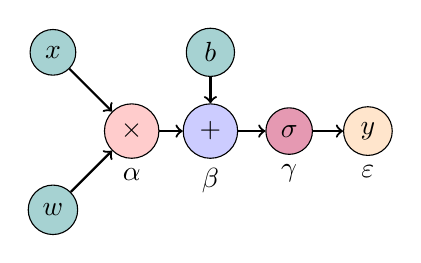
\begin{tikzpicture}[node distance=1cm]
    \node[draw, circle, fill=red!20, label=below:$\alpha$] (multiply) {$\times$};
    \node[draw, circle, fill=blue!20, right of=multiply, label=below:$\beta$] (addition) {$+$};
    \node[draw, circle, fill=purple!40, right of=addition, label=below:$\gamma$] (function) {$\sigma$};
    \node[draw, circle, fill=orange!20, right of=function, label=below:$\varepsilon$] (output) {$y$};

    \draw[->, thick] (multiply) -- (addition);
    \draw[->, thick] (addition) -- (function);
    \draw[->, thick] (function) -- (output);

    \node[draw, circle, fill=teal!35, left of=multiply, yshift=1cm] (input1) {$x$};
    \node[draw, circle, fill=teal!35, left of=multiply, yshift=-1cm] (input2) {$w$};
    \node[draw, circle, fill=teal!35, left of=addition, yshift=1cm, xshift=1cm] (bias) {$b$};

    \draw[->, thick] (input1) -- (multiply);
    \draw[->, thick] (input2) -- (multiply);
    \draw[->, thick] (bias) -- (addition);
\end{tikzpicture}
\caption{Computational graph of a feed forward pass of a simple neural network as in \eqref{eq:supersimple_NN}, adapted from \cite{autodiff}.}
\label{fig:forward_compgraph}
\end{figure}

Say we are interested in computing the derivative of $y$ with respect to the bias $b$, $\frac{\partial y}{\partial b}$.
As $y$ is not directly dependent on $b$, we compute the derivatives backward, as illustrated in \autoref{fig:backward_compgraph}, through extensive utilization of the chain rule.
We compute the derivatives with respect to each intermediate function through the chain rule, as
\begin{equation}
    \frac{\partial \varepsilon}{\partial b} = \frac{\partial \beta}{\partial b} \frac{\partial \varepsilon}{\partial \beta} = 
    \frac{\partial \beta}{\partial b}
    \frac{\partial \gamma}{\partial \beta}
    \frac{\partial \varepsilon}{\partial \gamma}.
\end{equation}
For one derivative, this is not particularly impressive.

\begin{figure}[h]
\centering
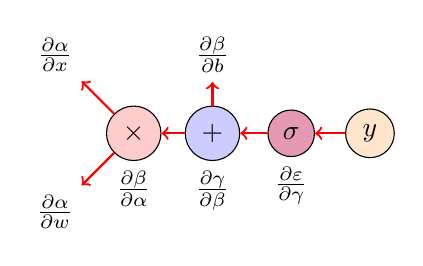
\begin{tikzpicture}[node distance=1cm]
    \node[draw, circle, fill=red!20, label=below:$\frac{\partial \beta}{\partial \alpha}$] (multiply) {$\times$};
    \node[draw, circle, fill=blue!20, right of=multiply, label=below:$\frac{\partial\gamma}{\partial\beta}$] (addition) {$+$};
    \node[draw, circle, fill=purple!40, right of=addition, label=below:$\frac{\partial \varepsilon}{\partial \gamma}$] (function) {$\sigma$};
    \node[draw, circle, fill=orange!20, right of=function] (output) {$y$};

    \draw[<-, thick, red] (multiply) -- (addition);
    \draw[<-, thick, red] (addition) -- (function);
    \draw[<-, thick, red] (function) -- (output);

    \node[left of=multiply, yshift=1cm,] (input1) {$\frac{\partial \alpha}{\partial x}$};
    \node[left of=multiply, yshift=-1cm,] (input2) {$\frac{\partial \alpha}{\partial w}$};
    \node[left of=addition, yshift=1cm, xshift=1cm,] (bias) {$\frac{\partial \beta}{\partial b}$};

    \draw[<-, thick, red] (input1) -- (multiply);
    \draw[<-, thick, red] (input2) -- (multiply);
    \draw[<-, thick, red] (bias) -- (addition);
\end{tikzpicture}
\caption{Automatic differentiation of a simple neural network as in \eqref{eq:supersimple_NN}, adapted from \cite{autodiff}.}
\label{fig:backward_compgraph}
\end{figure}

However, if we are next interested in computing the derivatives with respect to the other variables, we already have $\frac{\partial \varepsilon}{\partial \beta}$ computed.
This memoization is the reason automatic differentiation is able to compute derivatives efficiently, especially for functions with a larger number of inputs or outputs, e.g. a neural network with a large number of parameters.




